% !TeX document-id = {185283ec-c799-4d65-8857-a5189f5ded21}
% !TeX program = xelatex
% !TeX TXS-program:bibliography = txs:///biber
\documentclass[11pt]{article}

\usepackage{amsmath}
\usepackage{amsfonts}
\usepackage{amssymb}
\usepackage{amsthm}
\usepackage{graphicx}
\usepackage{booktabs}
\usepackage[usenames,dvipsnames]{xcolor}
\usepackage{tikz}
\usetikzlibrary{arrows,backgrounds}
\usepackage{hyperref}
\usepackage{caption}

% --- Chinese character support ---
% scheme=plain loads font support without imposing Chinese document
% conventions (section naming, date format, indentation). Without it, ctex
% renames the proof environment to 证明, which is wrong in an English paper.
\usepackage[scheme=plain]{ctex}
\renewcommand{\proofname}{Proof}   % belt and braces

\hypersetup{colorlinks=true,linkcolor=blue!55!black,citecolor=blue!55!black,
	urlcolor=blue!55!black}

\pagestyle{plain}
\textheight235truemm\textwidth165truemm
\voffset-2.2cm\hoffset-1.2cm \vfuzz=10000truept\hfuzz=10000truept

\newcommand{\RED}[1]{{\color{red}{#1}}}
\newcommand{\R}{{\mathbb{R}}}
\newcommand{\Z}{{\mathbb{Z}}}

\newtheorem{theorem}{Theorem}[section]
\newtheorem{lemma}[theorem]{Lemma}
\newtheorem{proposition}[theorem]{Proposition}
\newtheorem{corollary}[theorem]{Corollary}
\theoremstyle{definition}
\newtheorem{definition}[theorem]{Definition}
\theoremstyle{remark}
\newtheorem{remark}[theorem]{Remark}

\tikzstyle{place}=[circle,draw=blue!50,fill=blue!20,thick]

\usepackage[backend=biber,style=alphabetic,sorting=ynt]{biblatex}
\addbibresource{Chinese_med.bib}

\title{Saturating Interactions and the Stability of the Synchronous Equilibrium\\
	in the Five-Element Model of Traditional Chinese Medicine}
\author{Carter Feng and Yunjiao Wang}

\begin{document}
	\maketitle
	
	\begin{abstract}
		Continuous-time models of the five-element (Wu-Xing) network of Traditional Chinese
		Medicine have almost without exception represented the inter-organ interactions by
		bilinear terms, following the Lotka--Volterra formalism of population dynamics. We
		show that this choice determines the qualitative dynamics: under bilinear coupling
		the fully synchronous equilibrium, which is the natural dynamical representation of
		health, is generically unstable. We propose an alternative in which the generating
		and over-acting interactions are saturating, each term being derived from a named
		classical relation, and analyse the resulting system. The positive orthant is
		forward invariant and a compact box is globally attracting for all parameter values,
		so that positivity and boundedness hold without restriction. The system is
		equivariant under the cyclic group $\Z_5$, whence the Jacobian at a synchronous
		equilibrium is circulant and its spectrum is obtained in closed form by discrete
		Fourier transform. This yields a necessary and sufficient condition for asymptotic
		stability consisting of three inequalities, whose coefficients are the golden ratio
		and its reciprocal, and which distinguishes the synchronous isotypic component from
		the symmetry-breaking ones. Numerical evaluation of the criterion indicates that
		stability is lost exclusively through symmetry-breaking modes, by a Hopf bifurcation
		whose critical eigenspace supports discrete rotating waves. In the complementary
		parameter regime the system is bistable, the synchronous equilibrium being
		annihilated in a saddle-node bifurcation whose locus is obtained explicitly, so that
		the loss of stability is discontinuous and exhibits hysteresis. An extension
		incorporating a demand term and a counter-acting term reproduces the classical
		pathological relations 母病及子, 子盗母气, 相乘 and 相侮,
		together with the classical ordering of the two abnormal control relations.
	\end{abstract}
	
	\tableofcontents
	\newpage
	
	% ============================================================================
	\section{Introduction}\label{sec:intro}
	% ============================================================================
	
	Traditional Chinese Medicine (TCM) represents the body as a network of interacting
	organ systems rather than as a collection of independent
	organs~\cite{Kaptchuk2000,Tang2008}. The five-element, or Wu-Xing, diagram places
	five such systems on a cycle of generation (Sheng, 生) and a pentagram of
	control (Ke, 克). Diagnostic and therapeutic principles are formulated directly
	in terms of these two relations: the precept 虚则补其母, that a deficient child
	is treated by tonifying its mother, refers to a single edge of the generating cycle,
	and the abnormal relations 相乘 and 相侮 refer to single edges of the
	control cycle~\cite{NeiJing}. Porkert observed that Chinese medicine is not less
	logical than Western medicine but less analytical~\cite{Porkert1990}; the present
	work is concerned with the consequences of formulating these relations as a
	dynamical system.
	
	Existing quantitative treatments are of two kinds. Discrete models assign to each
	organ finitely many states, either active and inactive in a synchronous Boolean
	network~\cite{Bellavite1998} or excess, normal and deficiency~\cite{Chen2002}, or
	else reason algebraically about the relations without
	integration~\cite{MengYinYang,Zhang2011,Kim2014,Feng2003}. The asymptotic behaviour
	of such models is necessarily a fixed point or a cycle, so questions of asymptotic
	stability in the sense considered here do not arise. Continuous models assign to each
	organ a real-valued activity governed by an ordinary differential equation. A small
	number employ linear interaction terms~\cite{ChenZhang2008,Zhao2006}; the majority
	employ bilinear terms of the form $\beta x_i x_j$, by analogy with Lotka--Volterra
	population dynamics~\cite{Wang2008,Ding2008,Chen2008,Yu2005,Jiang2006,Li1987,
		Zhang1998,Murray2002}. Models within this family differ principally in the number of
	influences retained. Lin and Han~\cite{Lin2020} enumerate six and construct a
	symmetric five-dimensional system containing all of them; Nian and Li~\cite{Nian2025}
	have recently examined bifurcations in a related system. The asymptotic behaviours
	reported include equilibria~\cite{Wang2008,Ding2008,Chen2008,Yu2005}, periodic
	orbits~\cite{Jiang2006,Li1987,Zhang1998} and chaotic
	attractors~\cite{Jiang2006,Li1987}.
	
	The bilinear convention has two consequences that motivate the present work. First,
	in the terminology of population ecology a bilinear coupling is a Holling type~I
	functional response~\cite{Holling1959}, whose rate is unbounded in the interacting
	quantities. Second, it reverses the direction of one of the classical relations: the
	classical sources state that a deficient child draws more heavily upon its mother,
	whereas a term of the form $c\,x_i x_{\sigma(i)}$ tends to zero as the child is
	depleted. Both features are corrected by a saturating, or type~II, response. We
	establish that the substitution is not merely cosmetic: under bilinear coupling the
	synchronous equilibrium is generically unstable, so that the model admits no
	representation of sustained health, whereas under saturating coupling it is
	asymptotically stable on a substantial region of parameter space.
	
	The analysis is facilitated by the symmetry of the network. Since the five organs
	obey identical dynamical laws and the interaction structure is invariant under
	rotation by one position, the system is equivariant under the cyclic group $\Z_5$,
	and the Jacobian evaluated at a synchronous equilibrium is circulant. Its spectrum
	is therefore obtainable in closed form, and the isotypic decomposition separates the
	synchronous perturbations, under which all organs vary in unison, from the
	symmetry-breaking perturbations, under which they diverge. The latter correspond to
	the differentiated patterns of excess and deficiency identified in TCM diagnosis.
	
	The paper is organised as follows. Section~\ref{sec:model} formulates the model and
	derives each term from a named classical relation. Section~\ref{sec:basic}
	establishes forward invariance of the positive orthant, the existence of a globally
	attracting compact region, and the classification of synchronous equilibria.
	Section~\ref{sec:stability} derives the circulant structure of the Jacobian and the
	resulting stability criterion. Section~\ref{sec:bifurcation} identifies the
	codimension-one bifurcations by which the synchronous equilibrium is destabilised or
	annihilated. Section~\ref{sec:numerics} reports numerical simulations, including the
	reproduction of the classical pathological relations by an extended model.
	Section~\ref{sec:motifs} interprets the classical treatment principles in terms of
	network motifs, and Section~\ref{sec:discussion} discusses the scope and limitations
	of the results. Appendix~\ref{app:corrections} records corrections to Lyapunov
	spectra previously reported for the bilinear model, and
	Appendix~\ref{app:numerics} documents the numerical methods and their validation.
	
	% ============================================================================
	\section{Model formulation}\label{sec:model}
	% ============================================================================
	
	\subsection{The interaction network}
	
	The five organ systems are indexed according to the standard cycle:
	
	\begin{center}
		\begin{tabular}{cll}
			\toprule
			Index & Element & Organ \\
			\midrule
			$x_1$ & Wood\; (木) & Liver\; (肝) \\
			$x_2$ & Fire\; (火)  & Heart\; (心) \\
			$x_3$ & Earth\; (土) & Spleen\; (脾) \\
			$x_4$ & Metal\; (金) & Lung\; (肺) \\
			$x_5$ & Water\; (水) & Kidney\; (肾) \\
			\bottomrule
		\end{tabular}
	\end{center}
	
	Let $x_i(t)\ge0$ denote the functional activity, or qi, of organ $i$ at time $t$;
	indices are understood modulo five throughout. The generating cycle is
	$x_1\to x_2\to x_3\to x_4\to x_5\to x_1$, in which each organ is termed the
	\emph{mother} of its successor and the successor its \emph{child}. The control cycle
	follows the pentagram $x_1\dashv x_3\dashv x_5\dashv x_2\dashv x_4\dashv x_1$.
	Denoting by $\sigma(i)$ the mother of organ $i$, by $\kappa(i)$ the organ it
	controls, and by $\rho(i)$ the organ controlling it,
	\begin{equation}\label{eq:maps}
		\sigma(i)=i-1,\qquad \sigma^{-1}(i)=i+1,\qquad \kappa(i)=i+2,\qquad \rho(i)=i-2 .
	\end{equation}
	
	\begin{figure}[!htb]
		\centering
		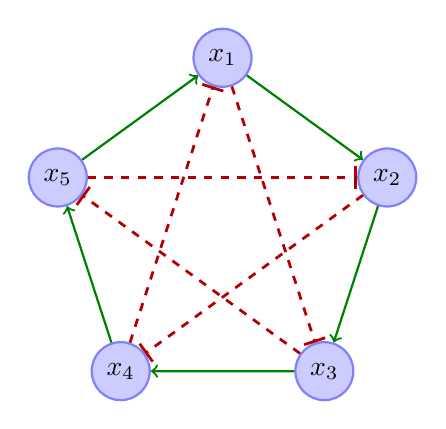
\begin{tikzpicture}[line width=1pt, scale=2.2]
			\node[place] (M) at (90:1) {$x_1$};
			\node[place] (H) at (18:1) {$x_2$};
			\node[place] (T) at (-54:1) {$x_3$};
			\node[place] (J) at (234:1) {$x_4$};
			\node[place] (S) at (162:1) {$x_5$};
			\path[->,green!50!black,thick]
			(M) edge (H) (H) edge (T) (T) edge (J) (J) edge (S) (S) edge (M);
			\path[-|,red!70!black,dashed]
			(M) edge (T) (T) edge (S) (S) edge (H) (H) edge (J) (J) edge (M);
		\end{tikzpicture}
		\caption{The Wu-Xing interaction network. Solid arrows denote the generating (Sheng)
			cycle; dashed bars denote the controlling (Ke) pentagram. Each organ possesses
			exactly one mother, one child, one controller and one target, and the configuration
			is invariant under rotation by one position.}
		\label{fig:network}
	\end{figure}
	
	\subsection{The classical relations}\label{sec:relations}
	
	The relations to be represented are those of the classical
	literature~\cite{NeiJing}, following the exposition
	of~\cite{Kaptchuk2000,Porkert1990}. Along the generating cycle, the mother nourishes
	the child and a deficient child draws more heavily upon her; deficiency in the
	mother induces deficiency in the child (母病及子) and excess induces excess; an
	excessive child overdraws from the mother (子盗母气); and sustained weakness in
	the child eventually depletes the mother. Along the control cycle, ordinary
	restraint is physiological and serves to prevent unbounded growth of the target;
	where the controller is excessive or the target deficient, the target is severely
	weakened, the relation termed 相乘 and classified as 贼邪, the ``thief
	evil''; and conversely, where the target is excessive or the controller deficient,
	the controller is mildly weakened, the relation termed 相侮 and classified as
	微邪, the ``mild evil''. The explicit ordering of these two abnormal relations
	constrains the corresponding coefficients and is used in
	Section~\ref{sec:pathologies}.
	
	\subsection{Governing equations}
	
	We consider the system
	\begin{equation}\label{eq:sat}
		\dot{x}_i \;=\;
		\underbrace{a x_i - k x_i^2}_{\text{self-regulation}}
		\;+\;\underbrace{\frac{c\,x_{\sigma(i)}}{1+x_i}}_{\text{generation}}
		\;-\;\underbrace{\frac{g\,x_i}{1+x_{\kappa(i)}}}_{\text{over-acting}}
		\;-\;\underbrace{h\,x_i x_{\rho(i)}}_{\text{restraint}},
		\qquad i\in\Z_5 ,
	\end{equation}
	with $a,k,c,g,h>0$. The four terms are derived as follows.
	
	The self-regulation term is logistic, comprising production proportional to current
	activity together with a quadratic limitation, and possesses intrinsic carrying
	capacity $a/k$.
	
	In the generation term, the numerator renders nourishment proportional to the
	mother's activity, so that deficiency and excess propagate from mother to child in
	accordance with the classical relations. The denominator represents demand: the
	factor $(1+x_i)^{-1}$ approaches unity as the child is depleted and decreases as the
	child becomes replete. This is the relation that a bilinear term cannot represent,
	since the product $c\,x_ix_{\sigma(i)}$ vanishes precisely in the limit of greatest
	need.
	
	The over-acting term represents 相乘. The factor $(1+x_{\kappa(i)})^{-1}$
	approaches unity when the controlled organ is deficient, so that the demand upon
	$x_i$ is then maximal, and decreases as the controlled organ approaches its normal
	level. Deficiency in the target thus amplifies the cost borne by the controller.
	
	The restraint term is retained in bilinear form. Ordinary suppression requires both
	parties to be present, and a product is therefore the appropriate representation. In
	the terminology of population ecology, the model replaces type~I functional
	responses by type~II responses on the generating and over-acting edges while
	retaining a type~I response on the restraint edge~\cite{Holling1959,Murray2002}.
	
	System~\eqref{eq:sat} omits the counter-acting relation 相侮 and the
	consumption borne by the mother. Both are reinstated in
	Section~\ref{sec:pathologies}, where they are shown to be required for the
	reproduction of the full set of classical pathologies. The reduced
	system~\eqref{eq:sat} is analysed first, being the smallest model exhibiting the
	phenomena under consideration; the analysis extends without modification.
	
	\begin{remark}[Scaling]\label{rem:scaling}
		The substitutions $t\mapsto at$ and $x\mapsto (a/k)x$ reduce the five parameters to
		three, at the cost of introducing an explicit scale into the saturation
		denominators, which become $1+(a/k)x_i$. Since the classical relations are expressed
		in terms of an organ being deficient or excessive relative to a fixed physiological
		norm, the dimensional form is retained, the saturation threshold furnishing the
		natural unit of activity and each coefficient retaining its interpretation. The
		values $a=2$, $k=0.5$, $c=1$, $g=0.5$ and $h=0.3$ are used throughout for
		illustration.
	\end{remark}
	% ============================================================================
	\section{Positivity, boundedness and equilibria}\label{sec:basic}
	% ============================================================================
	
	\subsection{Forward invariance and dissipativity}
	
	Since $x_i$ denotes a physiological activity, the model is admissible only if
	solutions remain nonnegative and bounded. For~\eqref{eq:sat} both properties hold
	without restriction on the parameters.
	
	\begin{proposition}[Invariant region]\label{prop:box}
		The positive orthant is forward invariant under~\eqref{eq:sat}, and the compact set
		$[0,X_{\max}]^5$ with
		\begin{equation}\label{eq:box}
			X_{\max}=\frac{a+\sqrt{a^{2}+4kc}}{2k}
		\end{equation}
		is positively invariant and globally attracting. In particular, no solution ceases
		to exist in finite time, for any admissible parameter values.
	\end{proposition}
	
	\begin{proof}
		Every term of~\eqref{eq:sat} contains a factor $x_i$ with the exception of the
		generation term, which is nonnegative. Hence $\dot x_i\ge0$ whenever $x_i=0$, and
		the boundary of the positive orthant cannot be crossed from within.
		
		For the second assertion, set $X(t)=\max_i x_i(t)$ and let $i$ attain the maximum.
		The generation term satisfies $c\,x_{\sigma(i)}/(1+x_i)\le cX/(1+X)<c$, while the
		over-acting and restraint terms are nonpositive. Therefore
		\[
		\dot X\;\le\;aX-kX^{2}+c ,
		\]
		and the right-hand side is negative whenever $kX^{2}-aX-c>0$, that is whenever
		$X>X_{\max}$ as given by~\eqref{eq:box}.
	\end{proof}
	
	The corresponding property fails for the bilinear model. Restricted to the
	synchronous subspace, that model reduces to $\dot x=ax-Mx^{2}$ with
	$M=b+d+g+h-c$, whose solutions cease to exist in finite time whenever $M<0$.
	Boundedness is thus a condition on the parameters rather than a structural property
	of the model, and the parameter values for which it fails are not excluded on
	physiological grounds.
	
	\subsection{Synchronous equilibria}
	
	\begin{definition}
		An equilibrium is \emph{synchronous} if $x_1=\cdots=x_5=x^\ast$. Synchronous
		equilibria with $x^\ast>0$ constitute the model's representation of health; the
		origin represents complete loss of function.
	\end{definition}
	
	Substituting $x_i=x^\ast$ into~\eqref{eq:sat}, every neighbour of every organ is
	equal to $x^\ast$ and the five equations reduce to one. Dividing by $x^\ast>0$ and
	clearing the denominator yields
	\begin{equation}\label{eq:quad}
		(k+h)\,(x^\ast)^{2} \;+\; \bigl[(k+h)-a\bigr]\,x^\ast \;-\;(a+c-g) \;=\; 0 .
	\end{equation}
	The leading coefficient being positive, the sign of the constant term $-(a+c-g)$
	determines the structure of the root set.
	
	\begin{proposition}\label{prop:exist}
		If $a+c>g$, equation~\eqref{eq:quad} possesses exactly one positive root,
		\begin{equation}\label{eq:xstar}
			x^\ast=
			\frac{\,a-(k+h)+\sqrt{\bigl[a-(k+h)\bigr]^{2}+4(k+h)(a+c-g)}\,}{2(k+h)},
		\end{equation}
		and system~\eqref{eq:sat} accordingly possesses a unique synchronous equilibrium in
		the interior of the positive orthant.
	\end{proposition}
	
	\begin{proof}
		The product of the roots of~\eqref{eq:quad} equals $-(a+c-g)/(k+h)$, which is
		negative under the stated hypothesis. Exactly one root is therefore positive, and it
		is given by~\eqref{eq:xstar}.
	\end{proof}
	
	The condition $a+c>g$ requires that self-production together with nourishment
	received exceed the cost of nourishing the child. At the illustrative parameter
	values it yields $x^\ast=\tfrac34+\tfrac{\sqrt{59}}4\approx2.6703$. The complementary
	regime is treated in Section~\ref{sec:bistability}, where it is shown to admit two
	positive synchronous equilibria rather than none.
	
	% ============================================================================
	\section{Linear stability of the synchronous equilibrium}\label{sec:stability}
	% ============================================================================
	
	\subsection{Equivariance and the circulant structure of the Jacobian}
	
	Let $\gamma$ denote the cyclic shift $(\gamma x)_i=x_{i-1}$ on $\R^5$. The
	maps~\eqref{eq:maps} commute with $\gamma$, and the five organs obey identical laws;
	consequently the vector field $F$ of~\eqref{eq:sat} satisfies
	$F(\gamma x)=\gamma F(x)$, so that~\eqref{eq:sat} is equivariant under the cyclic
	group $\Z_5=\langle\gamma\rangle$. Equivariance is inherited by the linearisation at
	any $\gamma$-invariant point, and every synchronous equilibrium is such a point.
	
	\begin{lemma}\label{lem:circulant}
		Let $J$ denote the Jacobian of~\eqref{eq:sat} at a synchronous equilibrium
		$x^\ast$, and set $s=1+x^\ast$. Then
		\[
		J_{ii}=a-2kx^\ast-\frac{cx^\ast}{s^{2}}-\frac{g}{s}-hx^\ast,
		\qquad
		\frac{\partial\dot x_i}{\partial x_{\sigma(i)}}=\frac{c}{s},
		\qquad
		\frac{\partial\dot x_i}{\partial x_{\kappa(i)}}=\frac{gx^\ast}{s^{2}},
		\qquad
		\frac{\partial\dot x_i}{\partial x_{\rho(i)}}=-hx^\ast,
		\]
		all remaining entries being zero, and $J$ is circulant.
	\end{lemma}
	
	\begin{proof}
		The partial derivatives are obtained by differentiating~\eqref{eq:sat} and
		evaluating at $x_i=x^\ast$ for all $i$; the two saturating terms require the
		quotient rule. The three nonzero off-diagonal entries occupy the positions
		$\sigma(i)=i-1$, $\kappa(i)=i+2$ and $\rho(i)=i-2$, which stand at offsets
		independent of $i$. Each row is therefore the preceding row advanced by one
		position, which is the definition of a circulant matrix.
	\end{proof}
	
	\subsection{Closed-form spectrum and stability criterion}
	
	Circulant matrices are diagonalised by the discrete Fourier basis~\cite{Davis1979}.
	Writing $\omega=e^{2\pi i/5}$, the eigenvalues of $J$ are the values of the symbol of
	its first row at the fifth roots of unity,
	\begin{equation}\label{eq:dft}
		\lambda_j=J_{ii}+\frac{gx^\ast}{s^{2}}\,\omega^{2j}-hx^\ast\,\omega^{3j}
		+\frac{c}{s}\,\omega^{4j},\qquad j=0,\dots,4 .
	\end{equation}
	Since $\omega^{3}=\overline{\omega^{2}}$ and $\omega^{4}=\overline{\omega}$, only two
	distinct cosines occur in the real parts, and both admit expression in terms of the
	golden ratio $\varphi=(1+\sqrt5)/2$:
	\[
	\cos\frac{2\pi}{5}=\frac{1}{2\varphi},\qquad
	\cos\frac{4\pi}{5}=-\frac{\varphi}{2} .
	\]
	
	\begin{theorem}\label{thm:criterion}
		Let $x^\ast>0$ be a synchronous equilibrium of~\eqref{eq:sat}, let $s=1+x^\ast$, and
		define
		\[
		D=a-2kx^\ast-\frac{cx^\ast}{s^{2}}-\frac{g}{s}-hx^\ast,
		\qquad
		T=x^\ast\Bigl(\frac{g}{s^{2}}-h\Bigr),
		\qquad
		M=\frac{c}{s} .
		\]
		Then $J$ possesses exactly three distinct eigenvalue real parts,
		\begin{equation}\label{eq:threemodes}
			\operatorname{Re}\lambda_{0}=D+T+M,
			\qquad
			\operatorname{Re}\lambda_{1,4}=D-\tfrac{\varphi}{2}T+\tfrac{1}{2\varphi}M,
			\qquad
			\operatorname{Re}\lambda_{2,3}=D+\tfrac{1}{2\varphi}T-\tfrac{\varphi}{2}M,
		\end{equation}
		and $x^\ast$ is asymptotically stable if and only if all three are negative.
	\end{theorem}
	
	\begin{proof}
		Taking real parts in~\eqref{eq:dft} gives
		$\operatorname{Re}\lambda_j=D+T\cos(4\pi j/5)+M\cos(8\pi j/5)$, the contributions of
		the target and controller combining because $\cos(6\pi j/5)=\cos(4\pi j/5)$ for
		every $j$. Evaluation of the cosines at $j=0,\dots,4$ yields only the values $1$,
		$1/(2\varphi)$ and $-\varphi/2$, arranged as stated. The equivalence of asymptotic
		stability with negativity of all eigenvalue real parts at a hyperbolic equilibrium
		is standard.
	\end{proof}
	
	At the illustrative parameter values, \eqref{eq:threemodes} gives
	$\operatorname{Re}\lambda_0\approx-2.2353$,
	$\operatorname{Re}\lambda_{1,4}\approx-1.1537$ and
	$\operatorname{Re}\lambda_{2,3}\approx-2.2432$, so that the synchronous equilibrium is
	asymptotically stable. For the bilinear model at the parameter values
	of~\cite{Lin2020}, the corresponding computation yields the pair
	$0.206\pm0.634i$, of positive real part, and the synchronous equilibrium is
	unstable. Figure~\ref{fig:eig} displays the two spectra.
	
	\begin{figure}[!htb]
		\centering
		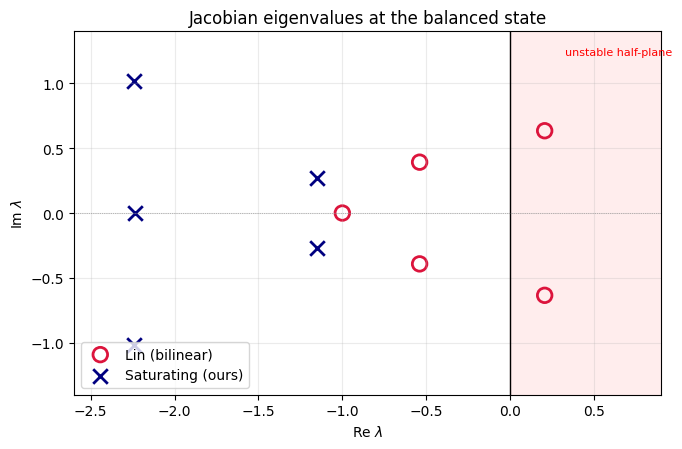
\includegraphics[width=0.66\textwidth]{fig1_eigenvalues.png}
		\caption{Spectra of the Jacobian at the synchronous equilibrium of each model. The
			shaded half-plane is the region of positive real part. Two of the five bilinear
			eigenvalues lie within it; all five eigenvalues of the saturating model lie strictly
			to the left of the imaginary axis.}
		\label{fig:eig}
	\end{figure}
	
	\subsection{Isotypic decomposition}\label{sec:modes}
	
	The three expressions in~\eqref{eq:threemodes} correspond to the isotypic components
	of the $\Z_5$ action. The mode $j=0$ has eigenvector $(1,1,1,1,1)$ and spans the
	synchronous subspace; a perturbation in this direction alters the activity of all
	five organs equally, leaving them mutually balanced. The modes $j=1,\dots,4$, which
	occur in complex-conjugate pairs, span the complementary symmetry-breaking subspace;
	perturbations in these directions differentiate the organs, producing a pattern of
	excess and deficiency across the network. The latter correspond to the differentiated
	patterns identified in TCM diagnosis, and which of the three conditions
	in~\eqref{eq:threemodes} is violated first therefore determines the character of the
	resulting disorder.
	
	The three conditions weight $T$ and $M$ differently. The synchronous mode
	superposes both at unit weight, whereas the symmetry-breaking modes oppose them with
	weights $-\varphi/2$ and $1/(2\varphi)$. An increase in the restraint coefficient $h$
	renders $T$ more negative, which relaxes the condition for $j=1,4$ and tightens that
	for $j=2,3$; the resulting competition determines the stability boundary.
	% ============================================================================
	\section{Bifurcation analysis}\label{sec:bifurcation}
	% ============================================================================
	
	The synchronous equilibrium may cease to be an asymptotically stable representation
	of health in three distinct ways, each admitting an explicit condition. Two concern
	its existence and follow from the quadratic~\eqref{eq:quad}; the third concerns its
	stability and follows from Theorem~\ref{thm:criterion}.
	
	\subsection{Transcritical bifurcation at the origin}
	
	The origin is an equilibrium of~\eqref{eq:sat} for all parameter values, and its
	stability admits a closed-form characterisation.
	
	\begin{proposition}\label{prop:origin}
		The Jacobian of~\eqref{eq:sat} at the origin is $J(0)=(a-g)I+cP$, where $P$ is the
		permutation matrix of the map $\sigma$. Its eigenvalues are
		$\lambda_j=(a-g)+c\,\omega^{j}$ for $j=0,\dots,4$, whence the spectral abscissa is
		$a+c-g$ and the origin is asymptotically stable if and only if $a+c<g$.
	\end{proposition}
	
	\begin{proof}
		At $x=0$ one has $s=1$, so that the diagonal entries of Lemma~\ref{lem:circulant}
		reduce to $a-g$, and the entries associated with the target and controller vanish,
		each containing a factor $x^\ast$. Only the entry $c$ in the position $\sigma(i)$
		survives, whence $J(0)=(a-g)I+cP$. The eigenvalues of the cyclic permutation $P$ are
		the fifth roots of unity, and $\operatorname{Re}\omega^{j}=\cos(2\pi j/5)$ attains
		its maximum at $j=0$.
	\end{proof}
	
	The condition of Proposition~\ref{prop:origin} is the negation of that of
	Proposition~\ref{prop:exist}. The two results are therefore complementary: for
	$a+c>g$ the origin is unstable and a unique positive synchronous equilibrium exists,
	while for $a+c<g$ the origin is asymptotically stable. At $a+c=g$ the positive branch
	passes through the origin and the two equilibria exchange stability, which is a
	transcritical bifurcation.
	
	\subsection{Saddle-node bifurcation and bistability}\label{sec:bistability}
	
	For $a+c<g$ the constant term of~\eqref{eq:quad} is positive and its two roots are
	of like sign. Their sum is $[a-(k+h)]/(k+h)$, which is positive when $a>k+h$.
	Failure of the condition $a+c>g$ therefore does not imply that the origin is the
	only nonnegative equilibrium; for $a>k+h$ there may exist two positive synchronous
	equilibria.
	
	\begin{proposition}\label{prop:fold}
		Let $a>k+h$. The discriminant of~\eqref{eq:quad} vanishes at
		\begin{equation}\label{eq:gfold}
			g=g_{\mathrm f}:=a+c+\frac{\bigl[a-(k+h)\bigr]^{2}}{4(k+h)},
		\end{equation}
		where the two positive roots coalesce at
		$x^\ast_{\mathrm f}=[a-(k+h)]/[2(k+h)]$. For $a+c<g<g_{\mathrm f}$ there exist two
		positive synchronous equilibria and for $g>g_{\mathrm f}$ none, so that the system
		undergoes a saddle-node bifurcation at $g=g_{\mathrm f}$.
	\end{proposition}
	
	\begin{proof}
		The discriminant of~\eqref{eq:quad} is $[a-(k+h)]^{2}+4(k+h)(a+c-g)$. Setting it
		equal to zero and solving for $g$ yields~\eqref{eq:gfold}, and the repeated root is
		$-B/(2A)$ with $A=k+h$ and $B=(k+h)-a$.
	\end{proof}
	
	Evaluation of the spectrum on each branch yields the configuration characteristic of
	a saddle-node bifurcation: the upper branch is asymptotically stable, the lower is of
	saddle type, and by Proposition~\ref{prop:origin} the origin is asymptotically stable
	throughout the interval. The system is accordingly bistable for
	$a+c<g<g_{\mathrm f}$, the lower branch constituting the separatrix between the two
	basins of attraction. Figure~\ref{fig:bistability} displays the bifurcation diagram
	together with two solutions initiated on either side of the separatrix.
	
	\begin{figure}[!htb]
		\centering
		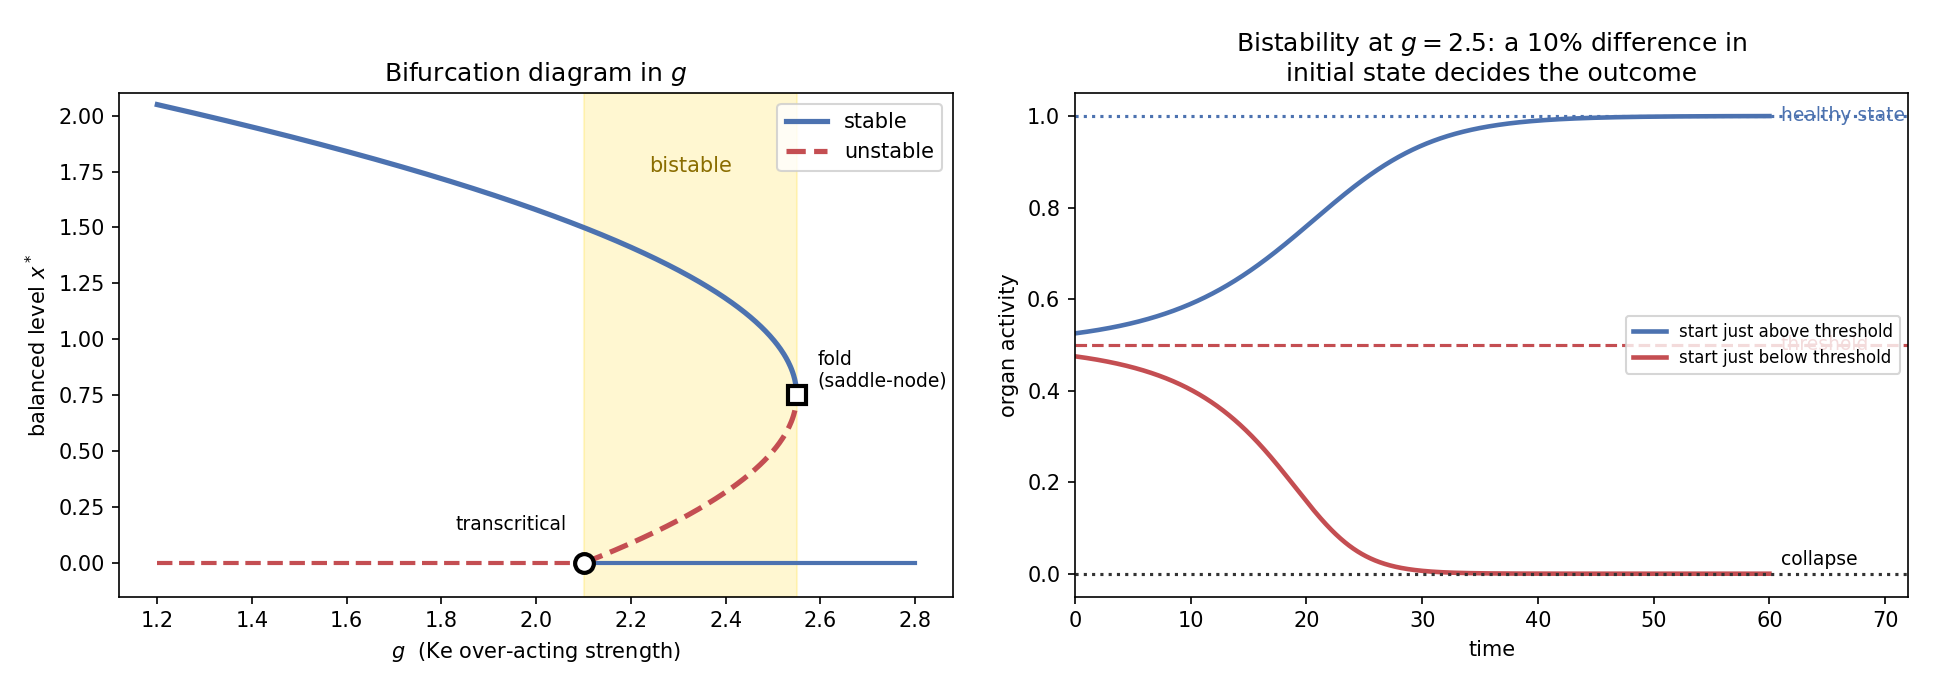
\includegraphics[width=\textwidth]{P5_bistability.png}
		\caption{Left: bifurcation diagram in the over-acting coefficient $g$ for $a=2$,
			$k=0.5$, $c=0.1$ and $h=0.3$. Solid curves denote asymptotically stable equilibria
			and dashed curves unstable ones. The upper branch is annihilated at
			$g_{\mathrm f}=2.55$ at the finite value $x^\ast=0.75$, and the shaded interval is
			bistable. Right: two solutions within that interval, initiated ten percent above and
			ten percent below the separatrix, converging respectively to the positive
			equilibrium and to the origin.}
		\label{fig:bistability}
	\end{figure}
	
	Three consequences follow. Within the bistable interval the asymptotic state is
	determined by the initial condition rather than by the parameters, so that systems
	with identical parameter values may converge either to the positive equilibrium or
	to the origin according to their position relative to the separatrix. The positive
	branch is not attenuated continuously but annihilated at a finite value of $x^\ast$,
	so that a slow variation of $g$ through $g_{\mathrm f}$ produces a discontinuous
	loss of function. Since the origin remains asymptotically stable throughout the
	interval, reversal of that variation does not restore the system to the positive
	branch; recovery requires either reduction of $g$ below the transcritical value or a
	perturbation returning the state to the basin of the positive equilibrium. The
	transition therefore exhibits hysteresis.
	
	\subsection{Symmetry-breaking Hopf bifurcation}\label{sec:hopf}
	
	Where the positive synchronous equilibrium exists it may nonetheless lose stability
	through violation of Theorem~\ref{thm:criterion}, and the isotypic component in
	which the violation occurs determines the character of the bifurcation.
	
	Evaluating~\eqref{eq:threemodes} on a $200\times200$ grid in the generation
	coefficient $c$ and the restraint coefficient $h$, the synchronous mode $j=0$ is
	critical in three percent of grid cells, and at each of the $680$ cells lying within
	$0.02$ of the stability boundary the critical eigenvalues are the pair $j=1,4$
	(Figure~\ref{fig:criticalmode}). Within the region examined, the synchronous
	equilibrium therefore does not lose stability through a synchronous perturbation. A
	synchronous instability would correspond to uniform depletion or uniform
	over-activity with the organs remaining mutually balanced; the computation indicates
	instead that stability is lost through a differentiated pattern of excess and
	deficiency, which is the form in which TCM diagnosis is expressed. This is a
	consequence of the symmetry of the network rather than an assumption of the model.
	
	\begin{figure}[!htb]
		\centering
		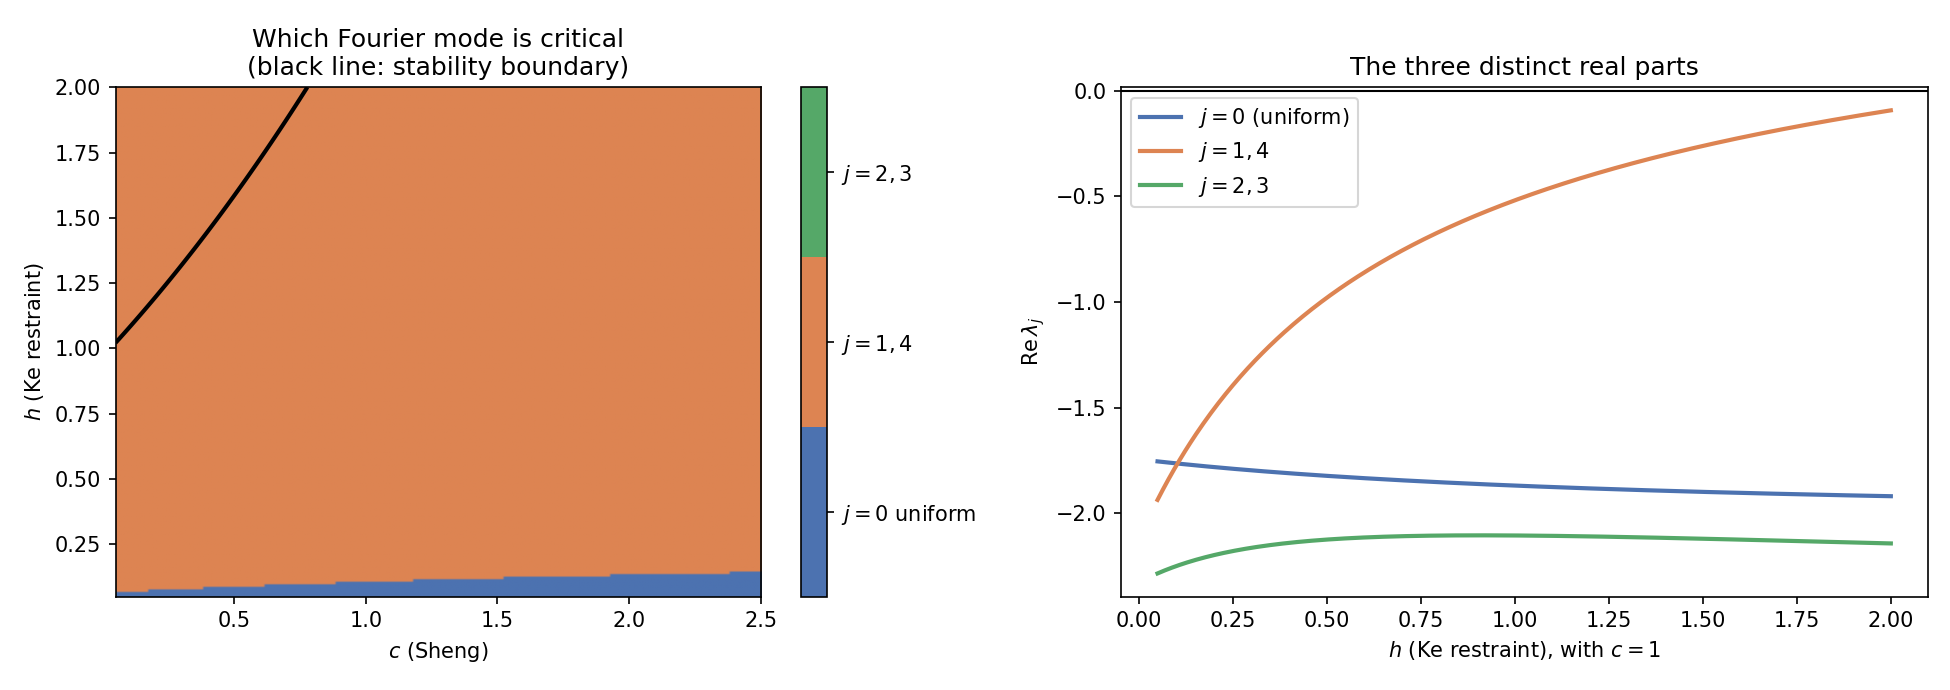
\includegraphics[width=\textwidth]{P4_critical_mode.png}
		\caption{Left: the critical isotypic component across the $(c,h)$ plane, with the
			stability boundary superimposed. Right: the three eigenvalue real parts
			of~\eqref{eq:threemodes} along the section $c=1$, showing the pair $j=1,4$ crossing
			the imaginary axis while the synchronous mode remains strictly negative.}
		\label{fig:criticalmode}
	\end{figure}
	
	Since $j=1,4$ is a complex-conjugate pair, the crossing is oscillatory provided the
	imaginary part is nonzero at criticality. Bisection in $h$ at $a=1.5$, $k=0.65$,
	$c=1$ and $g=0.5$ locates the boundary at $h_{c}=2.3718$, where $x^\ast=0.5998$ and
	the spectrum is
	\[
	\pm0.310613\,i,\qquad -1.929714,\qquad -2.158417\pm1.831876\,i ,
	\]
	a single conjugate pair on the imaginary axis with the remaining eigenvalues of
	negative real part. The transversality and nondegeneracy conditions being satisfied
	generically, the transition is a Hopf bifurcation, and the period of the emergent
	oscillation at onset is $2\pi/|\operatorname{Im}\lambda|=20.23$. Repetition of the
	bisection at other values of $c$ yields the same classification throughout, the
	imaginary part decreasing as $c$ increases (Table~\ref{tab:hopf}).
	
	\begin{table}[!htb]
		\centering
		\begin{tabular}{ccc}
			\toprule
			$c$ & $h_{c}$ & critical pair \\
			\midrule
			$0.5$ & $1.5843$ & $\pm0.4113\,i$ \\
			$1.0$ & $2.3718$ & $\pm0.3106\,i$ \\
			$1.5$ & $3.3475$ & $\pm0.1976\,i$ \\
			$2.0$ & $4.0000$ & $\pm0.0790\,i$ \\
			\bottomrule
		\end{tabular}
		\caption{The stability boundary at several values of the generation coefficient. In
			each case a single complex-conjugate pair crosses the imaginary axis with nonzero
			imaginary part.}
		\label{tab:hopf}
	\end{table}
	
	The critical eigenspace being a symmetry-breaking isotypic component of a
	$\Z_5$-equivariant system, the equivariant Hopf theorem predicts branches of
	discrete rotating waves, in which the organs oscillate with a constant phase lag of
	one fifth of the period~\cite{GolubitskyStewartSchaeffer1988,GolubitskyStewart2002}.
	Periodic solutions of this form have been reported for bilinear
	models~\cite{Lin2020}, which suggests that the two formulations lose stability into
	solutions of the same isotropy type notwithstanding their different couplings. The
	criticality of the bifurcation is determined by the first Lyapunov coefficient,
	which has not been computed here; the distinction is material, since a subcritical
	Hopf bifurcation would render the onset of oscillation discontinuous and hysteretic
	in the manner of the saddle-node bifurcation of Section~\ref{sec:bistability}.
	
	% ============================================================================
	\section{Numerical simulations}\label{sec:numerics}
	% ============================================================================
	
	\subsection{Response to perturbation of a single organ}
	
	Theorem~\ref{thm:criterion} concerns infinitesimal perturbations. To assess its
	consequences for perturbations of finite magnitude, solutions were initiated at the
	synchronous equilibrium with a single organ displaced, and the deviation
	$\|x(t)-x^\ast\mathbf 1\|_2$ recorded.
	
	\begin{figure}[!htb]
		\centering
		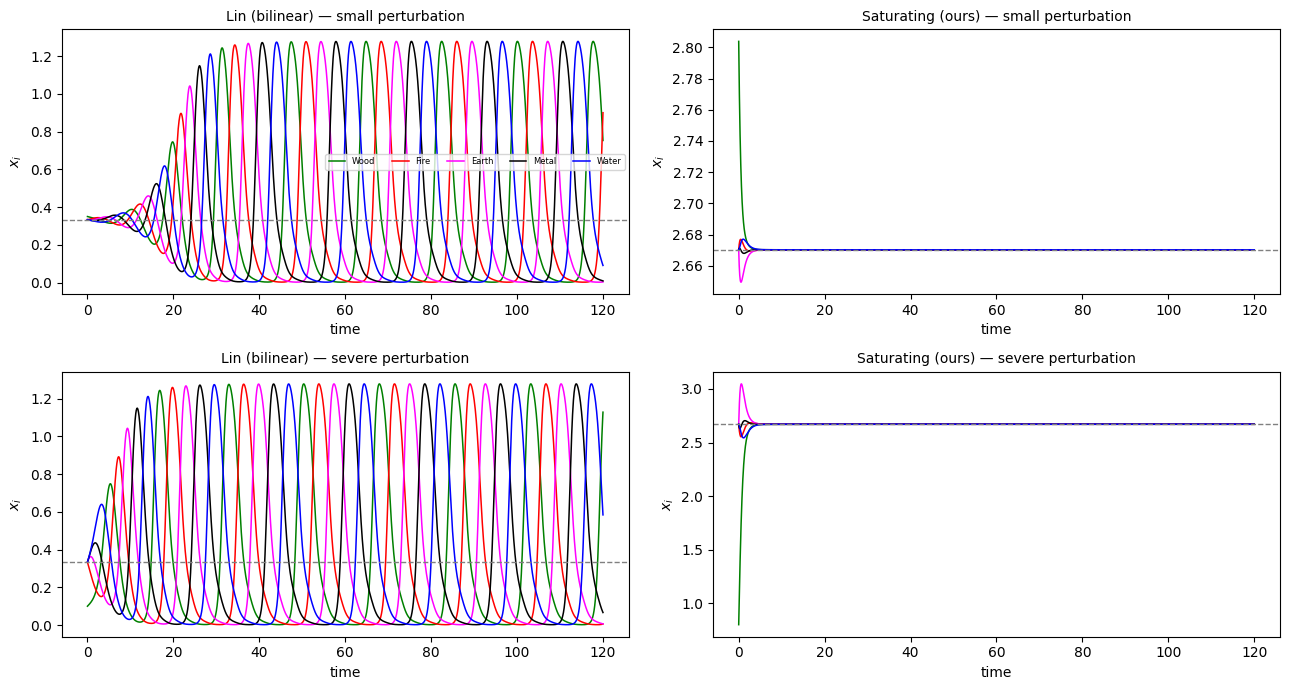
\includegraphics[width=\textwidth]{fig2_perturbation.png}
		\caption{Response to displacement of a single organ by five percent (upper row) and
			to thirty percent of the equilibrium value (lower row). The dashed line marks the
			synchronous equilibrium.}
		\label{fig:pert}
	\end{figure}
	
	In the saturating model the deviation decays to zero following both a five percent
	displacement and a severe deficiency. In the bilinear model a five percent
	displacement is amplified by a factor of approximately fifty, and a severe deficiency
	drives several organs towards zero. Since the interaction structure is invariant
	under rotation, displacement of any organ must produce an identical response; this
	was verified, the responses agreeing across the five choices to within $10^{-14}$
	(Figure~\ref{fig:z5}). The agreement also constitutes a consistency check on the
	implementation of the maps~\eqref{eq:maps}, an error in which would break the
	equivariance.
	
	\begin{figure}[!htb]
		\centering
		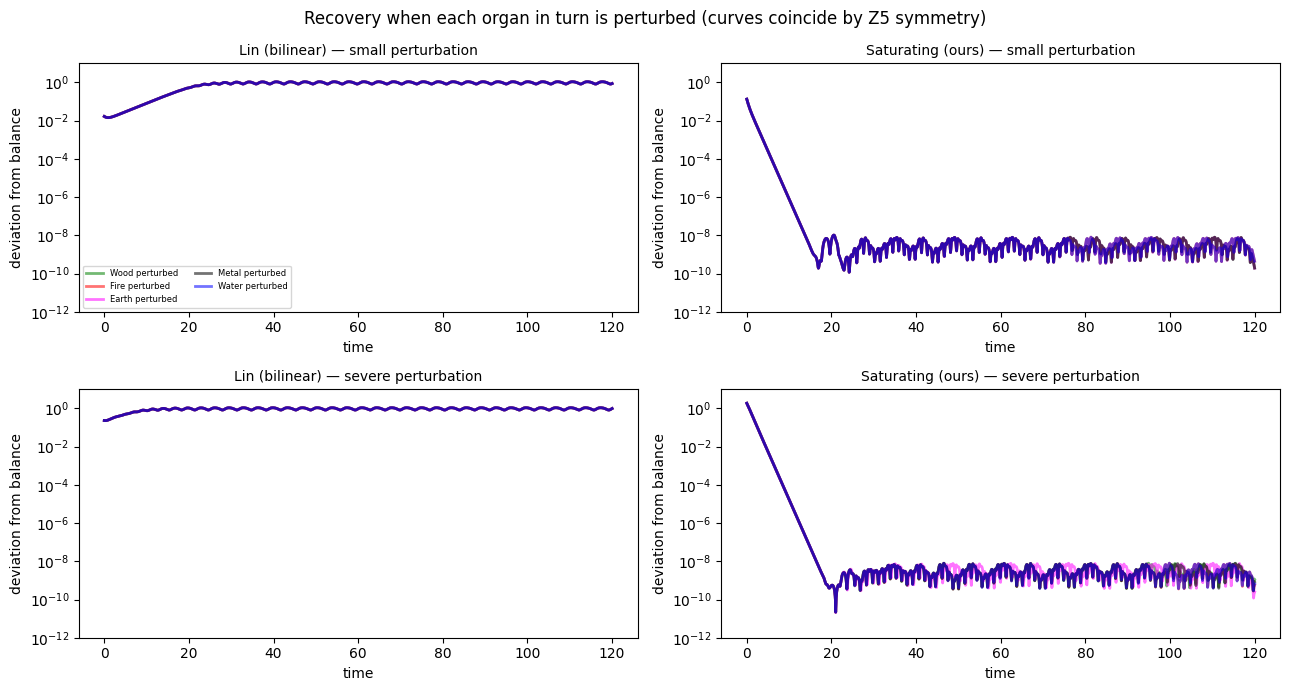
\includegraphics[width=\textwidth]{fig3_perturbation_all_organs.png}
		\caption{Deviation from the synchronous equilibrium, on a logarithmic scale,
			following displacement of each organ in turn. The five curves coincide, as
			equivariance requires. In the saturating model the deviation decays by eight orders
			of magnitude before reaching the tolerance of the integrator.}
		\label{fig:z5}
	\end{figure}
	
	\subsection{Extent of the region of stability}\label{sec:extent}
	
	Theorem~\ref{thm:criterion} determines stability at a given point of parameter
	space but not the measure of the stable set, which depends upon the distribution
	assumed over the coefficients. Figure~\ref{fig:stabmap} evaluates the criterion
	across the plane of generation against restraint: the saturating model is stable
	throughout the region shown, the bilinear model on less than one fifth of it.
	
	\begin{figure}[!htb]
		\centering
		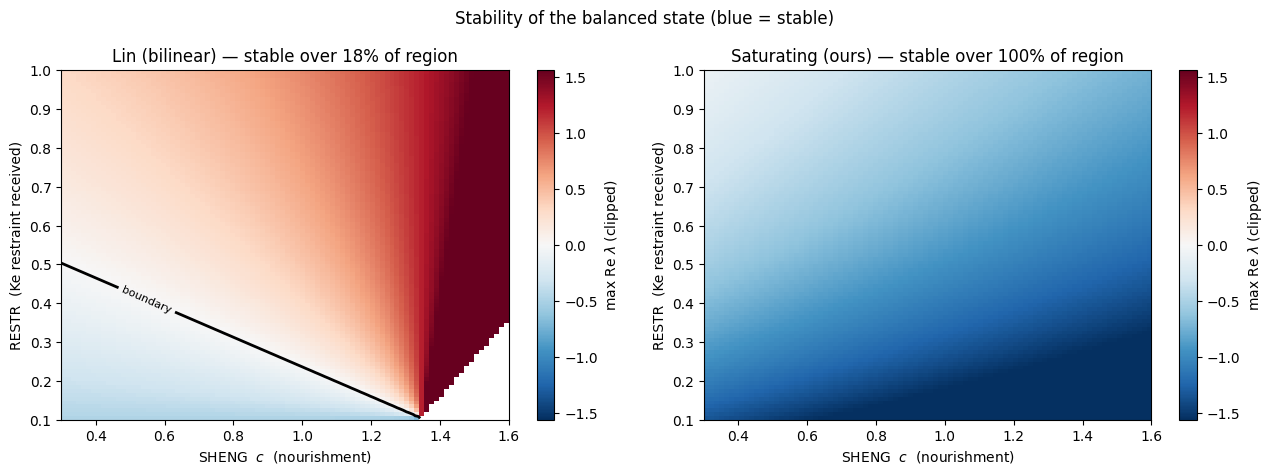
\includegraphics[width=\textwidth]{fig4_stability_maps.png}
		\caption{Spectral abscissa at the synchronous equilibrium across the $(c,h)$ plane,
			the remaining coefficients being held at mid-range values. Blue denotes asymptotic
			stability. The pale region in the left panel is that in which the bilinear model
			possesses no positive synchronous equilibrium.}
		\label{fig:stabmap}
	\end{figure}
	
	To establish that this is not an artefact of the particular section, coefficients
	were additionally sampled at random. No canonical distribution over them being
	available, three were used: independent uniform variates; variates conditioned on
	the ordering $\texttt{SELF}>\texttt{SHENG}>\texttt{RESTR}>\texttt{TGT}$, under which
	self-production exceeds generation, generation exceeds ordinary restraint, and
	ordinary restraint exceeds over-acting; and variates drawn from intervals assigned
	to each quantity in accordance with that ordering. Draws for which a model possesses
	no positive synchronous equilibrium are excluded from the corresponding count, each
	model being assessed only where it is well posed. The resulting proportions of
	stable draws are $22.8\%$, $47.1\%$ and $23.3\%$ for the bilinear model, against
	$94.1\%$, $91.9\%$ and $99.0\%$ for the saturating model, the Wilson intervals being
	disjoint in each case.
	
	The imposition of the ordering approximately doubles the proportion for the bilinear
	model while slightly reducing that for the saturating model; the conditioned
	distribution is therefore the more favourable to the bilinear formulation, and the
	comparison under it the more conservative. It should further be noted that the two
	models do not possess the same number of coefficients, the bilinear model carrying
	an additional term representing the cost of nourishing the child. Removal of that
	term reduces its stable proportion from $22.1\%$ to $12.0\%$, so that the asymmetry
	operates in favour of the bilinear model.
	
	\subsection{Reproduction of the classical pathological relations}\label{sec:pathologies}
	
	The foregoing results are dynamical. We now assess whether the model reproduces the
	pathological relations enumerated in Section~\ref{sec:relations}.
	
	A chronic disorder is represented by a sustained modification of the self-production
	coefficient of a single organ, $a_j=\lambda a$, with $\lambda=0.4$ representing
	deficiency and $\lambda=1.6$ excess. The system is integrated to its new asymptotic
	state and the relative change in each organ recorded.
	
	Applied to~\eqref{eq:sat}, this procedure reproduces 母病及子, 相乘 and
	相侮, but not 子盗母气: rendering the child excessive increases the
	mother by $12.9\%$. The discrepancy has a structural origin. In the Wu-Xing topology
	the control target of Fire is Metal, and Metal is the controller of Wood, so that
	$\kappa(2)=4=\rho(1)$. An excess of Fire consequently suppresses Metal, and the
	suppression of Metal relieves Wood of restraint, so that Wood increases. The excess
	of the child thus reaches the mother along two paths of opposite sign, and the
	classical relation asserts that the direct path predominates; a model omitting that
	path necessarily obtains the opposite sign.
	
	The construction of the omitted term requires care. A term of conservation type,
	$-g_s x_i/(1+x_{\sigma^{-1}(i)})$, representing the transfer received by the child,
	is decreasing in the child's activity and therefore cannot represent an excessive
	child consuming more. The relation 子盗母气 describes demand rather than
	conservation, and is represented by
	\[
	-\,\frac{g_d\,x_{\sigma^{-1}(i)}\,x_i}{1+x_i},
	\]
	in which the loss borne by the mother increases with the activity of the child.
	
	\begin{remark}
		The classical statements exhibit a tension at this point. A deficient child is said
		to draw more heavily upon its mother, while an excessive child is said to overdraw
		from her; the two assertions are opposed in direction and cannot proceed from a
		single term. We interpret them as describing distinct mechanisms, namely a
		physiological demand for nourishment, represented by the factor $(1+x_i)^{-1}$ in
		the generation term, and a pathological over-consumption, represented by the term
		above. The extended model contains both.
	\end{remark}
	
	Incorporating the demand term together with the counter-acting term of
	Section~\ref{sec:relations} yields
	\begin{equation}\label{eq:ext}
		\dot{x}_i =
		a_i x_i - k x_i^2
		+\frac{c\,x_{\sigma(i)}}{1+x_i}
		-\frac{g_d\,x_{\sigma^{-1}(i)}\,x_i}{1+x_i}
		-\frac{g\,x_i}{1+x_{\kappa(i)}}
		-h\,x_i x_{\rho(i)}
		-\frac{b\,x_{\kappa(i)}}{1+\epsilon x_i} .
	\end{equation}
	Both additional terms are nonpositive and both are defined through the
	maps~\eqref{eq:maps}. Proposition~\ref{prop:box} and Lemma~\ref{lem:circulant}
	therefore apply without modification: system~\eqref{eq:ext} remains positive,
	dissipative and $\Z_5$-equivariant, and its Jacobian at a synchronous equilibrium
	remains circulant.
	
	\begin{table}[!htb]
		\centering
		\begin{tabular}{llll r}
			\toprule
			Relation & Modification & Organ specified & Predicted & Observed \\
			\midrule
			母病及子 & Wood deficient  & Fire (child)      & decrease          & $-19.3\%$ \\
			子盗母气 & Fire excessive  & Wood (mother)     & decrease          & $-6.1\%$  \\
			相乘     & Wood excessive  & Earth (target)    & marked decrease   & $-31.3\%$ \\
			相侮     & Earth excessive & Wood (controller) & slight decrease   & $-17.7\%$ \\
			\bottomrule
		\end{tabular}
		\caption{Classical pathological relations reproduced by~\eqref{eq:ext} at
			$g_d=0.35$, $b=0.10$ and $\epsilon=0.5$.}
		\label{tab:pathologies}
	\end{table}
	
	\begin{figure}[!htb]
		\centering
		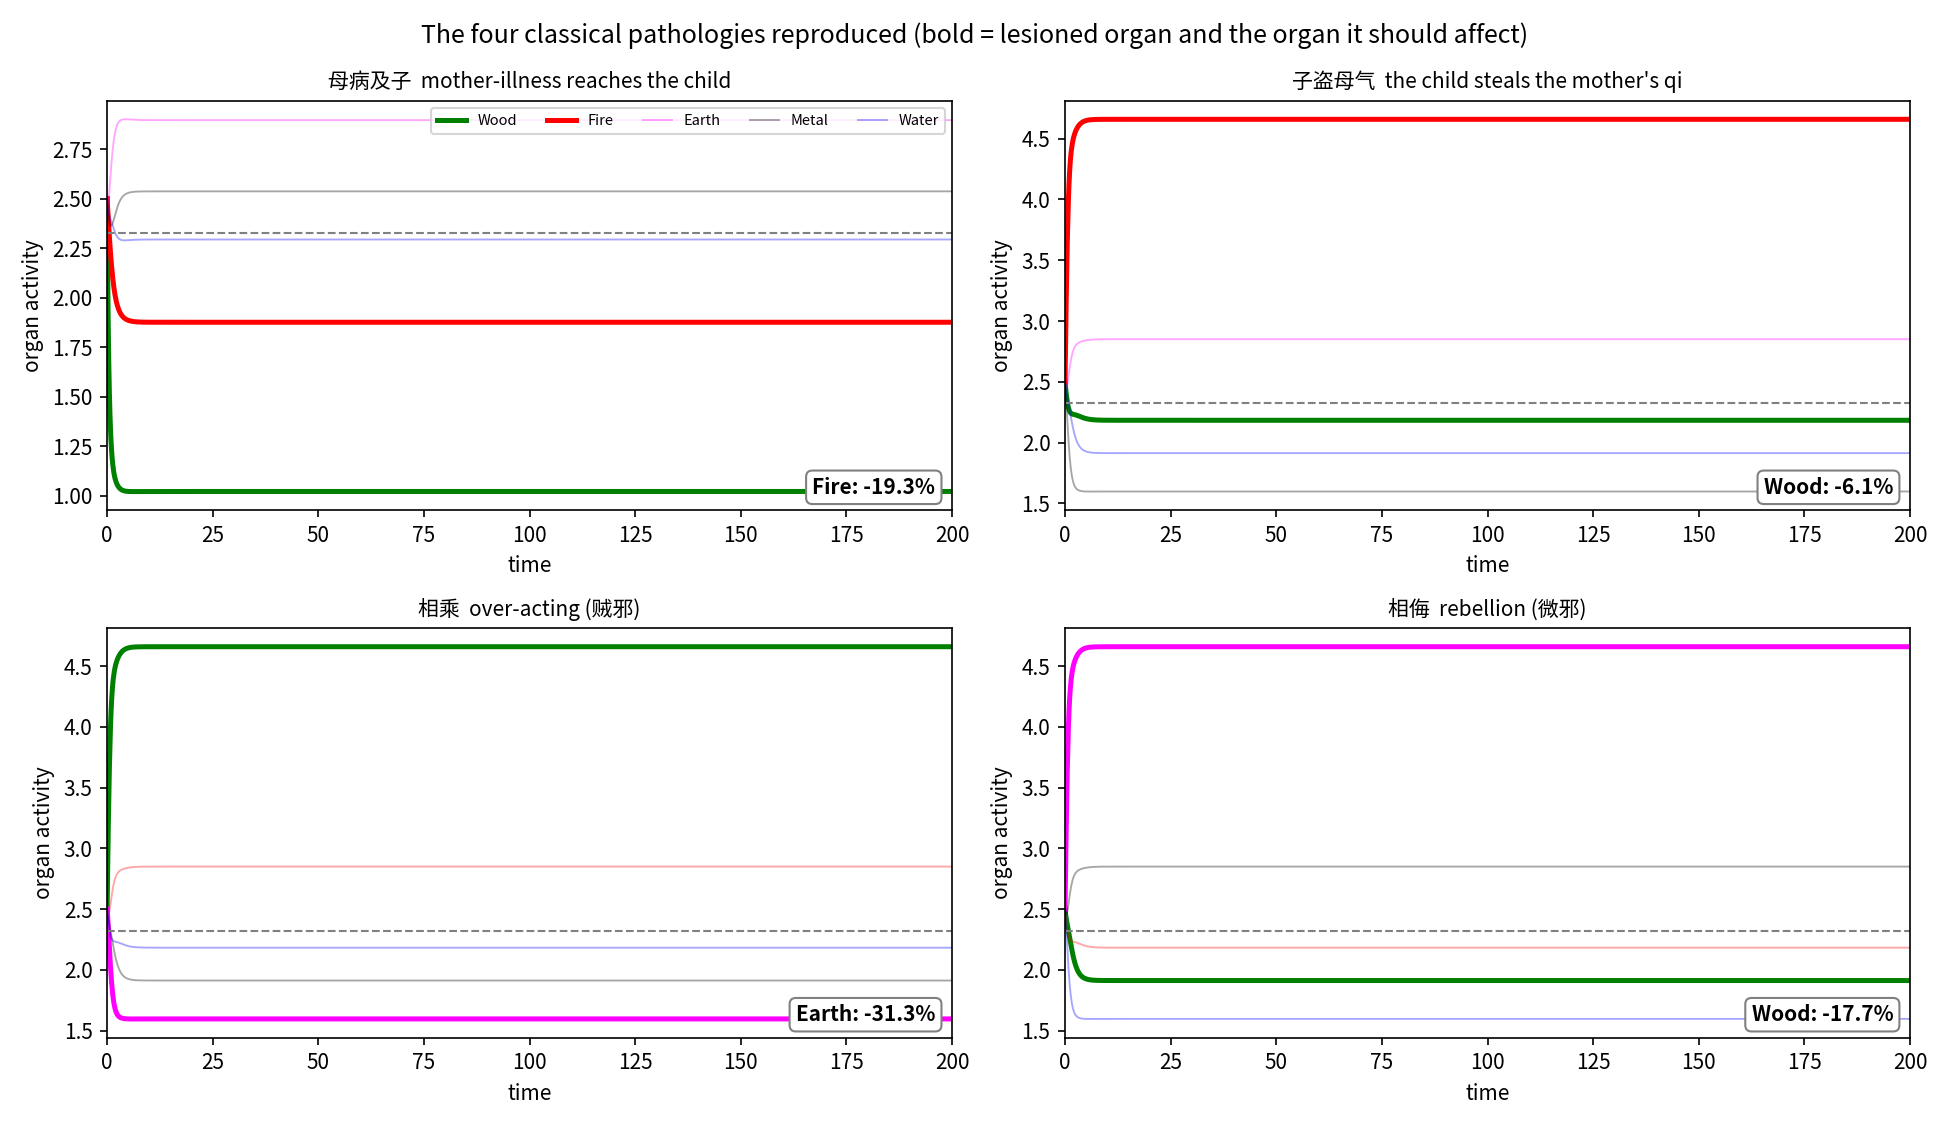
\includegraphics[width=\textwidth]{P1_pathologies.png}
		\caption{The four classical pathological relations. A single organ is modified at
			$t=0$ and the system approaches a new asymptotic state; the dashed line marks the
			original synchronous equilibrium. The modified organ and the organ specified by the
			relation are drawn in bold.}
		\label{fig:pathologies}
	\end{figure}
	
	All four relations are reproduced with the correct sign, and the classical ordering
	is respected, the effect of 相乘 ($-31.3\%$) exceeding in magnitude that of
	相侮 ($-17.7\%$). A sweep of the two additional coefficients shows that all five
	criteria are satisfied simultaneously on $53\%$ of the region examined
	(Figure~\ref{fig:pathregion}), so that the agreement does not depend on a particular
	choice. The failures at the boundary of that region are informative: for $b$ large
	relative to $g_d$ the counter-acting effect exceeds the over-acting effect and the
	classical ordering is violated, while for $g_d$ small the demand of the child does
	not overcome the indirect control path and 子盗母气 fails. The classical
	statements therefore constrain the coefficients from both directions, and in
	particular require the counter-acting coefficient to be small, which is the content
	of its classification as 微邪.
	
	\begin{figure}[!htb]
		\centering
		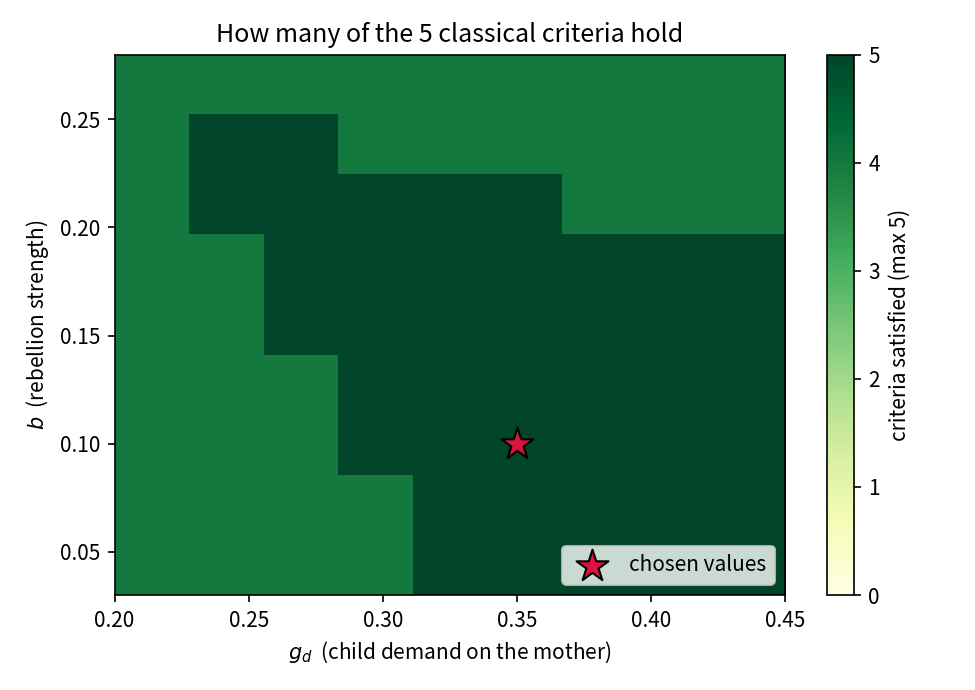
\includegraphics[width=0.6\textwidth]{P3_consistency_region.png}
		\caption{Number of the five classical criteria satisfied across the plane of the
			demand coefficient against the counter-acting coefficient. The marked point
			indicates the values of Table~\ref{tab:pathologies}.}
		\label{fig:pathregion}
	\end{figure}
	
	\begin{figure}[!htb]
		\centering
		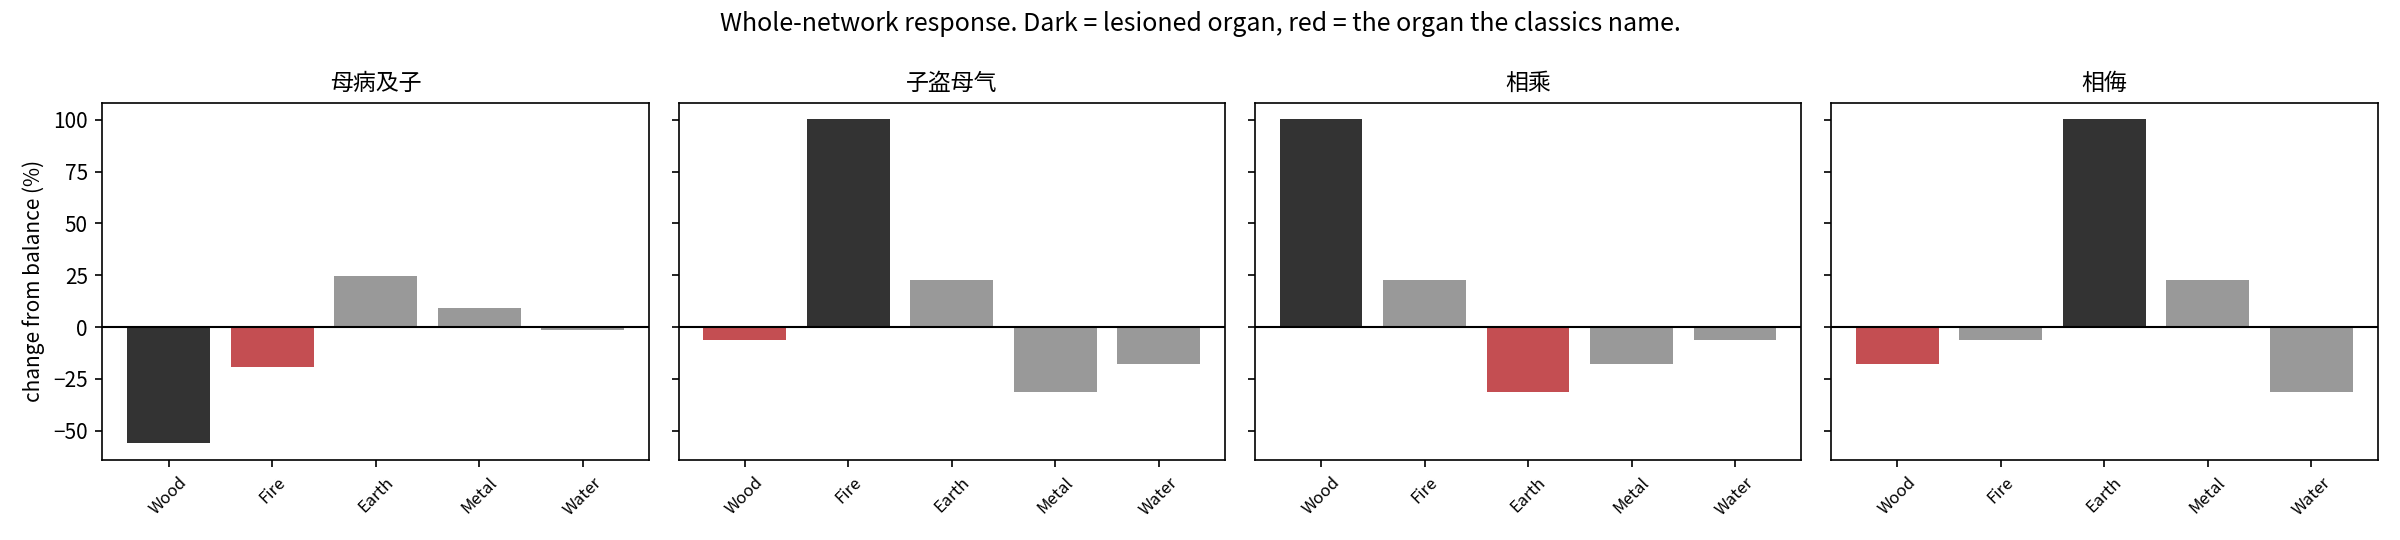
\includegraphics[width=\textwidth]{P2_network_response.png}
		\caption{Response of the entire network to each modification. Dark bars indicate the
			modified organ and light bars the organ specified by the classical relation.}
		\label{fig:pathnetwork}
	\end{figure}
	
	Figure~\ref{fig:pathnetwork} shows that the effect upon the organ specified by the
	classical relation is not in general the largest in the network, the control target
	of the modified organ being frequently displaced further. This is consistent with the
	classical emphasis upon the control cycle as the principal route of transmission, and
	with the corresponding therapeutic principle of protecting the organ next in that
	sequence rather than treating only the organ already affected.
	% ============================================================================
	\section{Network motifs}\label{sec:motifs}
	% ============================================================================
	
	\RED{[To be written. The argument to be developed: each classical therapeutic
		principle refers to only two or three organs---虚则补其母 and 实则泻其子
		refer to a single generating edge, 相乘 and 相侮 to a single control edge,
		and the principle of strengthening the organ next to be affected refers to a
		three-node configuration---so that TCM constitutes an implicit motif theory of
		physiology in the sense of~\cite{Milo2002,ShenOrr2002,Alon2007,AlonBook,Mangan2003}.
		Reasoning of this local character is justified precisely when the coupling to the
		remainder of the network is weak or slow by comparison with the dynamics internal to
		the motif, which is a statement concerning separation of time scales and is testable
		within the present model. The isotypic decomposition of Section~\ref{sec:modes}
		provides the connection between the local motifs and the global dynamics, each
		isotypic component being a delocalised pattern whose projection onto a given motif
		may be computed directly.]}
	
	% ============================================================================
	\section{Discussion}\label{sec:discussion}
	% ============================================================================
	
	The results presented above indicate that the functional form assumed for the
	inter-organ interactions determines whether the five-element system admits a
	representation of sustained health. Under bilinear coupling, nourishment is
	proportional to the product of the activities of mother and child. This reverses the
	classical relation, a depleted child then receiving less rather than more, and leaves
	the interaction unbounded, so that it may exceed the quadratic self-limitation. The
	synchronous equilibrium is in consequence unstable, and outside the region in which
	the loss coefficients dominate the gain, solutions cease to exist in finite time.
	Substitution of a saturating response corrects both features: the factor
	$(1+x_i)^{-1}$ renders nourishment greatest when the child is most depleted, and
	bounds the interaction, so that the quadratic term ultimately dominates. The
	consequences are the invariant region of Proposition~\ref{prop:box}, positivity and
	dissipativity independent of the parameters, and asymptotic stability of the
	synchronous equilibrium on a substantial region of parameter space.
	
	The circulant structure of the Jacobian is of interest beyond its computational
	convenience. The isotypic decomposition separates the synchronous component, in which
	the organs vary in unison, from the symmetry-breaking components, in which they are
	differentiated; the numerical evidence of Section~\ref{sec:hopf} indicates that
	stability is lost exclusively through the latter. The component in which the
	violation first occurs therefore determines the character of the resulting disorder,
	and the $\Z_5$ symmetry constrains the admissible patterns, predicting in particular
	discrete rotating waves at the Hopf bifurcation.
	
	Three limitations should be noted. First, the identification of health with a stable
	\emph{synchronous} equilibrium is an assumption. The physiological system is not
	exactly symmetric, and health might alternatively be represented by a bounded
	oscillation; the results establish that the saturating model admits a stable
	synchronous equilibrium where the bilinear model does not, and not that an
	equilibrium is the only admissible representation. Second,
	Theorem~\ref{thm:criterion} is a criterion for linear stability.
	Proposition~\ref{prop:box} furnishes an absorbing region and
	Section~\ref{sec:numerics} demonstrates recovery from perturbations of finite
	magnitude, but no Lyapunov function has been constructed and no claim of global
	asymptotic stability is made; indeed Section~\ref{sec:bistability} establishes that
	global stability fails on the bistable interval. Third, the coefficients of the
	extended system~\eqref{eq:ext} are constrained only by the qualitative classical
	statements and not by measurement, and the representation of a chronic disorder by a
	sustained modification of self-production is one modelling choice among several, the
	alternative of constraining an organ to a fixed level not having been examined.
	
	Several extensions suggest themselves. Computation of the first Lyapunov coefficient
	would determine the criticality of the Hopf bifurcation and hence whether the onset
	of oscillation is continuous. Two-parameter continuation of the stability boundary
	would locate the degenerate points at which the codimension-one bifurcations
	identified here interact. The intervention terms set to zero in~\cite{Lin2020} may be
	reinstated as control inputs, so that the model becomes a framework for the design of
	treatment: one then seeks the minimal intervention returning a diseased trajectory to
	the basin of attraction of the synchronous equilibrium, which corresponds to the
	classical principles of tonifying the mother and draining the child. Finally, the
	homeostatic target may be allowed to depend upon an organ's neighbours, through
	$\theta_i=\theta_i^0+\alpha_i x_{\sigma(i)}-\beta_i x_{\rho(i)}$, rendering
	homeostasis contextual rather than constitutional; the present analysis applies to
	that variant without modification.
	
	% ============================================================================
	\appendix
	% ============================================================================
	
	\section{Corrections to previously reported Lyapunov spectra}\label{app:corrections}
	
	The symmetric bilinear model of~\cite{Lin2020} was reimplemented in the course of
	this work, and its equilibria, its Jacobian eigenvalues to each published decimal,
	and its reported period $T\approx17.626$ were recovered. Three of the stability
	computations reported there do not, however, withstand examination, and the
	corrections are recorded here as they bear upon the stability of the bilinear
	synchronous equilibrium.
	
	\subsection*{A structural constraint upon Lyapunov spectra}
	
	For a smooth autonomous system $\dot x=F(x)$, differentiation of the equation with
	respect to $t$ gives $\tfrac{d}{dt}F(x(t))=DF(x)F(x)$, so that $v(t)=F(x(t))$ is a
	solution of the variational equation. Its Lyapunov exponent is
	$\lim_{t\to\infty}t^{-1}\log\|F(x(t))\|$, which vanishes whenever the orbit is
	bounded, $\|F\|$ then remaining within a compact interval bounded away from zero.
	Every bounded trajectory that is not an equilibrium therefore possesses an exponent
	equal to zero. The argument does not apply at an equilibrium, where $F=0$, which is
	why a stable equilibrium may possess only negative exponents. Both trajectories for
	which spectra are reported in~\cite{Lin2020} are bounded, one being a periodic orbit
	and the other confined by the invariants of Proposition~\ref{prop:conserved} below;
	both spectra must accordingly contain a zero exponent. Neither does:
	\[
	\{0.3885,-0.1719,-0.3473,-0.6833,-0.9731\}
	\quad\text{and}\quad
	\{0.6700,0.6606,-0.0761,-0.0794,-1.1751\}.
	\]
	
	\subsection*{The periodic orbit is asymptotically stable}
	
	Recomputation at $a=b=c=d=g=h=1$ by the variational method of Benettin et
	al.~\cite{Benettin1980a,Benettin1980b}, with periodic $QR$ reorthonormalisation and
	the initial transient discarded, yields
	$\{0.0011,-0.1232,-0.2721,-0.2728,-0.9998\}$: one zero exponent and four negative,
	which is the spectrum of an asymptotically stable limit cycle and not of the
	unstable periodic solution reported. The discrepancy is attributable to the
	singular-value method of~\cite{ZhangSVD2005}, employed in~\cite{Lin2020}
	following~\cite{Wolf1985}, having been applied over an interval including the
	transient, so that the rate of transient decay is measured in place of the
	asymptotic rate.
	
	\subsection*{The equilibrium is neutrally stable}
	
	For the case in which only the restraining influences are retained, the reported
	exponents $\{0.0015,0.0006,-1.3159,-2.3517,-3.7092\}$ were interpreted as containing
	two positive values. Evaluation of the Jacobian at the attained final state
	$(0,0,0,2.3426,1.3038)$ yields instead $\{0,0,-1.3038,-2.3426,-3.6464\}$, the two
	zeros being exact, coordinates resting at $x_i=0$ generating degenerate directions.
	The three negative eigenvalues agree with the reported values to within one percent,
	which identifies the reported positive entries as numerical error of order
	$10^{-3}$. The correct conclusion is neutral stability, consistent with the observed
	convergence of the trajectory; as published, the case is described simultaneously as
	convergent and unstable.
	
	\subsection*{The chaotic case is quasiperiodic}
	
	For $c=g=1$ and $a=b=d=h=0$ the bilinear model reduces to
	\begin{equation}\label{eq:conserv}
		\dot x_i=x_i(x_{i-1}-x_{i+1}),\qquad i\in\Z_5 .
	\end{equation}
	
	\begin{proposition}\label{prop:conserved}
		System~\eqref{eq:conserv} admits the independent first integrals
		$I_1=\sum_i x_i$ and $I_2=\prod_i x_i$.
	\end{proposition}
	
	\begin{proof}
		Summation of~\eqref{eq:conserv} over $i$ causes the right-hand side to telescope,
		whence $\tfrac{d}{dt}\sum_i x_i=0$. On the positive orthant,
		$\tfrac{d}{dt}\log\prod_i x_i=\sum_i(x_{i-1}-x_{i+1})=0$.
	\end{proof}
	
	Both integrals were confirmed numerically, the relative drift being of order
	$10^{-15}$. Two independent first integrals confine the motion to a
	three-dimensional invariant manifold, and the flow being volume-preserving, no
	attractor exists. The largest exponent computed over increasing intervals takes the
	values $0.0120$, $0.0070$ and $0.0038$ at $T=500$, $1000$ and $2000$, halving as $T$
	doubles, which is the behaviour of an exponent converging to zero rather than to the
	reported value $0.67$. The motion is quasiperiodic upon a torus.
	
	\subsection*{Consequence}
	
	The corrections do not affect the conclusion that the bilinear synchronous
	equilibrium is unstable, which follows from the eigenvalues $0.206\pm0.634i$
	reproduced exactly. They establish that its attracting sets are limit cycles or
	boundary equilibria at which several organs vanish, neither of which represents
	sustained health.
	
	\section{Numerical methods and validation}\label{app:numerics}
	
	Solutions were computed by adaptive Runge--Kutta methods and, in stiff regions, by
	LSODA, with relative and absolute tolerances of $10^{-9}$ and $10^{-11}$. Lyapunov
	spectra were computed by the variational method with periodic $QR$
	reorthonormalisation, an initial transient being discarded in each case. Bifurcation
	points were located by bisection upon the spectral abscissa and upon the
	discriminant of~\eqref{eq:quad}.
	
	Three independent checks were applied. The Jacobians of both models, obtained
	analytically, were compared with finite-difference approximations at random
	non-synchronous states, the largest discrepancies being $2.4\times10^{-7}$ and
	$3.2\times10^{-7}$ respectively, consistent with truncation error. The closed-form
	spectrum~\eqref{eq:threemodes} was compared with direct diagonalisation at $2582$
	randomly chosen parameter values, agreement being obtained to machine precision, and
	the stability classification derived from it agreed with that obtained numerically
	at all $2559$ parameter values admitting a synchronous equilibrium. Finally, the
	prediction of equivariance that displacement of any organ yields an identical
	response was verified to within $10^{-14}$, a discrepancy in which would indicate
	inconsistent implementation of the maps~\eqref{eq:maps}.
	
	\printbibliography
	
\end{document}